\documentclass{article}
\usepackage[a4paper,margin=3cm, total={6in, 9in}]{geometry}

\usepackage[utf8]{inputenc}
\usepackage{graphicx}
\graphicspath{ {./images/} }
\usepackage{float}

\usepackage{etoolbox}

\usepackage{amsmath}
\usepackage{circuitikz}
\usepackage{graphicx}

\makeatletter
\providecommand{\subtitle}[1]{% add subtitle to \maketitle
  \apptocmd{\@title}{\par {\large #1}}{}{}
}
\makeatother


\title{
\includegraphics[scale=0.65]{images/ozu.png}\\
\textbf{EE202 - Circuit Analysis}}
\subtitle{Laboratory #4}
\date{Fall 2022}
%\author{Laboratory 1}

\newcommand{\HRule}{\rule{\linewidth}{0.5mm}}

\begin{document}

\begin{titlepage}
\begin{center}

% Top 

\includegraphics[width=0.55\textwidth]{ozu.png}~\\[2cm]

% Title
\HRule \\[0.4cm]
{ \LARGE 
  \textbf{Lab Report for EE202 Circuit Analysis}\\[0.4cm]
  \emph{Laboratory 1}\\[0.4cm]
}
\HRule \\[1.5cm]

% Author
{ \large
  Ömer Faruk Avcı \\[0.1cm]
  \texttt{faruk.avci@ozu.edu.tr}
}

\vfill

%\textsc{\Large Cyprus University of Technology}\\[0.4cm]
\textsc{\large Department of Electrical and Electronics Engineering}\\[0.4cm]


% Bottom
{\large \today}
 
\end{center}
\end{titlepage}



\newpage

%\maketitle

\section{Introduction}
The lab consists of two main tasks: Task 1 focuses on determining voltage distribution in a voltage divider circuit using a voltmeter, measuring current flow, and comparing the results with theoretical values using KCL and KVL. Task 2 involves learning to configure an oscilloscope for voltage measurements and setting up a signal generator to supply sinusoidal voltages to the circuit.
\subsection{Preliminary Work}
{
The currents passing through each resistor are defined as follows:\begin{table}[h]
\begin{center}
\begin{tabular}{|c|c|}
\hline 
\textbf{Resistor ($R$)} & \textbf{Current ($i$)}  \\
\hline \hline
$R_1$ & $i_s$  \\ \hline
$R_2$ & $i_2$   \\  \hline
$R_3$ & $i_4$  \\ \hline
$R_4$ & $i_3$  \\ \hline
$R_5$ & $i_5$  \\ \hline
$R_6$ & $i_1$  \\ \hline
\end{tabular}
\caption{Resistors and current variables}
\end{center}
\end{table}

Using \textbf{Kirchhoff's Current Law(KCL)} and \textbf{Kirchhoff's Voltage Law (KVL)}, the following equations are obtained:
\begin{align}
  i_s - i_1 - i_2 - i_3 &= 0 \\  
  i_2 - i_4 - i_5 &= 0 \\  
  10\text{V} - 10\text{k} i_s - 10\text{k} i_3 &= 0 \\  
  10\text{k} i_3 - 33\text{k} i_2 - 33\text{k} i_5 &= 0 \\  
  33\text{k} i_5 - 47\text{k} i_4 &= 0 \\  
  -100\text{k} i_1 + 47\text{k} i_4 + 33\text{k} i_2 &= 0
\end{align}

Using the equations derived above, the system can be expressed in the form of a linear algebraic equation:
\begin{equation}
  \begin{bmatrix}
    1 & -1 & -1 & -1 &  0 &  0  \\
    0 &  0 &  1 &   0& -1 & -1  \\
   10\text{k} &  0 &  0 & 10\text{k} & 0 & 0  \\
    0 &  0 & -33\text{k} & 10\text{k} &  0 & -33\text{k}   \\
    0 &  0 &  0 &  0& -47\text{k} & 33\text{k}   \\
    0 & -100\text{k} & 33\text{k}& 0 & 47\text{k}  & 0
  \end{bmatrix}
  \begin{bmatrix}
    i_s  \\
    i_1  \\
    i_2  \\
    i_3  \\
    i_4  \\
    i_5  
  \end{bmatrix}
  =
  \begin{bmatrix}
    0  \\
    0  \\
    10\text{V}  \\
    0  \\
    0  \\
    0  
  \end{bmatrix}
\end{equation}


By solving the system of equations above using MATLAB, the currents through each resistor are obtained. These currents, when multiplied by the respective resistor values, yield the corresponding voltages across each resistor.


\begin{table}[ht]
\begin{center}
\begin{tabular}{|c|c|c|}
\hline 
\textbf{Resistor ($R$)} & \textbf{Current ($mA$)} & \textbf{Voltage ($V$)} \\
\hline \hline
$R_1 = 10\,\text{k}$ & $i_s = 0.5634$ & 5.63\\ \hline
$R_2 = 33\,\text{k}$ & $i_2 = 0.0833$ & 2.74 \\  \hline
$R_3 = 47\,\text{k}$ & $i_4 = 0.0343$ & 1.61 \\ \hline
$R_4 = 10\,\text{k}$ & $i_3 = 0.4365$ & 4.36 \\ \hline
$R_5 = 33\,\text{k}$ & $i_5 = 0.0489$ & 1.61 \\ \hline
$R_6 = 100\,\text{k}$ & $i_1 = 0.0436$& 4.36  \\ \hline
\end{tabular}
\caption{Current and Voltage values of resistors}
\end{center}
\end{table}
}

\newpage

\subsection{Lab Tasks}
\subsubsection{Task 1}

\begin{itemize}
  \item \textbf{Circuit Construction}


\begin{enumerate} 
  \item \textbf{Required Equipments:} 
  \begin{itemize} 
  \item 10V DC Power Supply 
  \item Breadboard 
  \item Jumper Cables (2) 
  \item 10k$\Omega$ Resistor (1) \item 33k$\Omega$ Resistors (2) 
  \item 47k$\Omega$ Resistor (1) \item 100k$\Omega$ Resistor (1) 
\end{itemize}

  \item \textbf{Simplified Circuit Schema}

  \begin{center}
    \begin{circuitikz}
        % Voltage source
        \draw (0,4) to[battery, l=10V] (0,0);

        \draw (0,4) to[R, l=$R_1$, a=$10\text{k}\Omega$] (3,4) 
        to[short] (3,4);
  
        \draw (3,4) to[short] (3,6)
        to[R,l=$R_6$,a=$100\text{k}\Omega$] (9,6)
        to[short] (10,6)
        to[short] (10,4);
  
        \draw (3,4) to[short] (3,4)
        to[R,l=$R_2$, a=$33\text{k}\Omega$] (5,4);
  
        \draw (5,4) to[short] (5,5)
        to[short] (6,5)
        to[R,l=$R_3$,a=$47\text{k}\Omega$] (8,5)
        to[short] (9,5)
        to[short] (9,4)
        to[short] (10,4);
  
        \draw (5,4) to[short] (5,3)
        to[short] (6,3)
        to[R, l=$R_5$,a=$33\text{k}\Omega$] (8,3)
        to[short] (9,3)
        to[short] (9,4);
  
  
        \draw (3,4) to[short](3,2)
        to[R,l=$R_4$,a=$10\text{k}\Omega$] (9,2)
        to[short] (10,2)
        to[short] (10,4);
        
        \draw (10,4) to[short] (11,4)
        to[short] (11,0)
        to[short] (0,0);
  
    \end{circuitikz}
    \end{center}
    
  Using the required components, a simplified version of the circuit can be efficiently assembled on the breadboard.

\end{enumerate}
\item \textbf{Measurement}
  
After constructing the circuit on the breadboard and turning on the power supplier, multimeter that is capable of measuring Voltage and Current is required to make the necessary measurements.

Using the probes of a multimeter, the measured voltages and currents passing through each resistor were determined. The results are summarized in the following table.

\begin{table}[h]
  \centering
  \begin{tabular}{|c|c|c|}
      \hline
      \textbf{Resistor} & \textbf{Current (mA)} & \textbf{Voltage (V)} \\
      \hline \hline
      $R_1$  & $i_s = 0.58$   & $V_{R1} = 5.59$ \\ \hline
      $R_2$  & $i_2 = 0.08$   & $V_{R2} = 2.71$ \\ \hline
      $R_3$  & $i_4 = 0.03$   & $V_{R3} = 1.62$ \\ \hline
      $R_4$  & $i_3 = 0.44$   & $V_{R4} = 4.37$ \\ \hline
      $R_5$  & $i_5 = 0.04$   & $V_{R5} = 1.62$ \\ \hline
      $R_6$  & $i_1 = 0.04$   & $V_{R6} = 4.37$ \\
      \hline
  \end{tabular}
  \caption{Measured Currents and Voltages for Each Resistor}
  \label{tab:measurements}
\end{table}


\end{itemize}


\subsubsection{Task 2}

\begin{enumerate}
    \item \textbf{Required Equipments:} 
    \begin{itemize} 
    \item Signal Generator 
    \item Oscilloscope 
    \item Breadboard 
    \item Jumper Cables (2) 
    \item 1k$\Omega$ Resistor (2) 
    \item 22k$\Omega$ Resistors (2) 
    \item 33k$\Omega$ Resistor (1) 
  \end{itemize}
  \item \textbf{Common Settings:} Before proceeding with the two subtasks, the following common settings should be applied to ensure consistency in measurements:
    \begin{itemize}
      \item The signal generator frequency should be set to \textbf{1 kHz}.

      \item The peak-to-peak voltage level should be adjusted to \textbf{2V}
    \end{itemize}
\end{enumerate}


\paragraph{1.2.2.1 Task 2.1}

Using the required equipment listed above, the circuit should be assembled using $ 1\text{k} \Omega $ resistors.

\begin{enumerate}
  \item[] \textbf{Measurement}
  \begin{itemize}
    \item The signal generator should be connected to the breadboard using its probes, and its output should be activated.  
    \item The oscilloscope probes should be properly connected to their designated measurement points in the circuit.  
    \item The oscilloscope display should be monitored to observe the channel waveforms and verify the expected signal behavior.  
    \item The observed waveform is presented in the following figure:
    \begin{figure}[h]
      \centering
      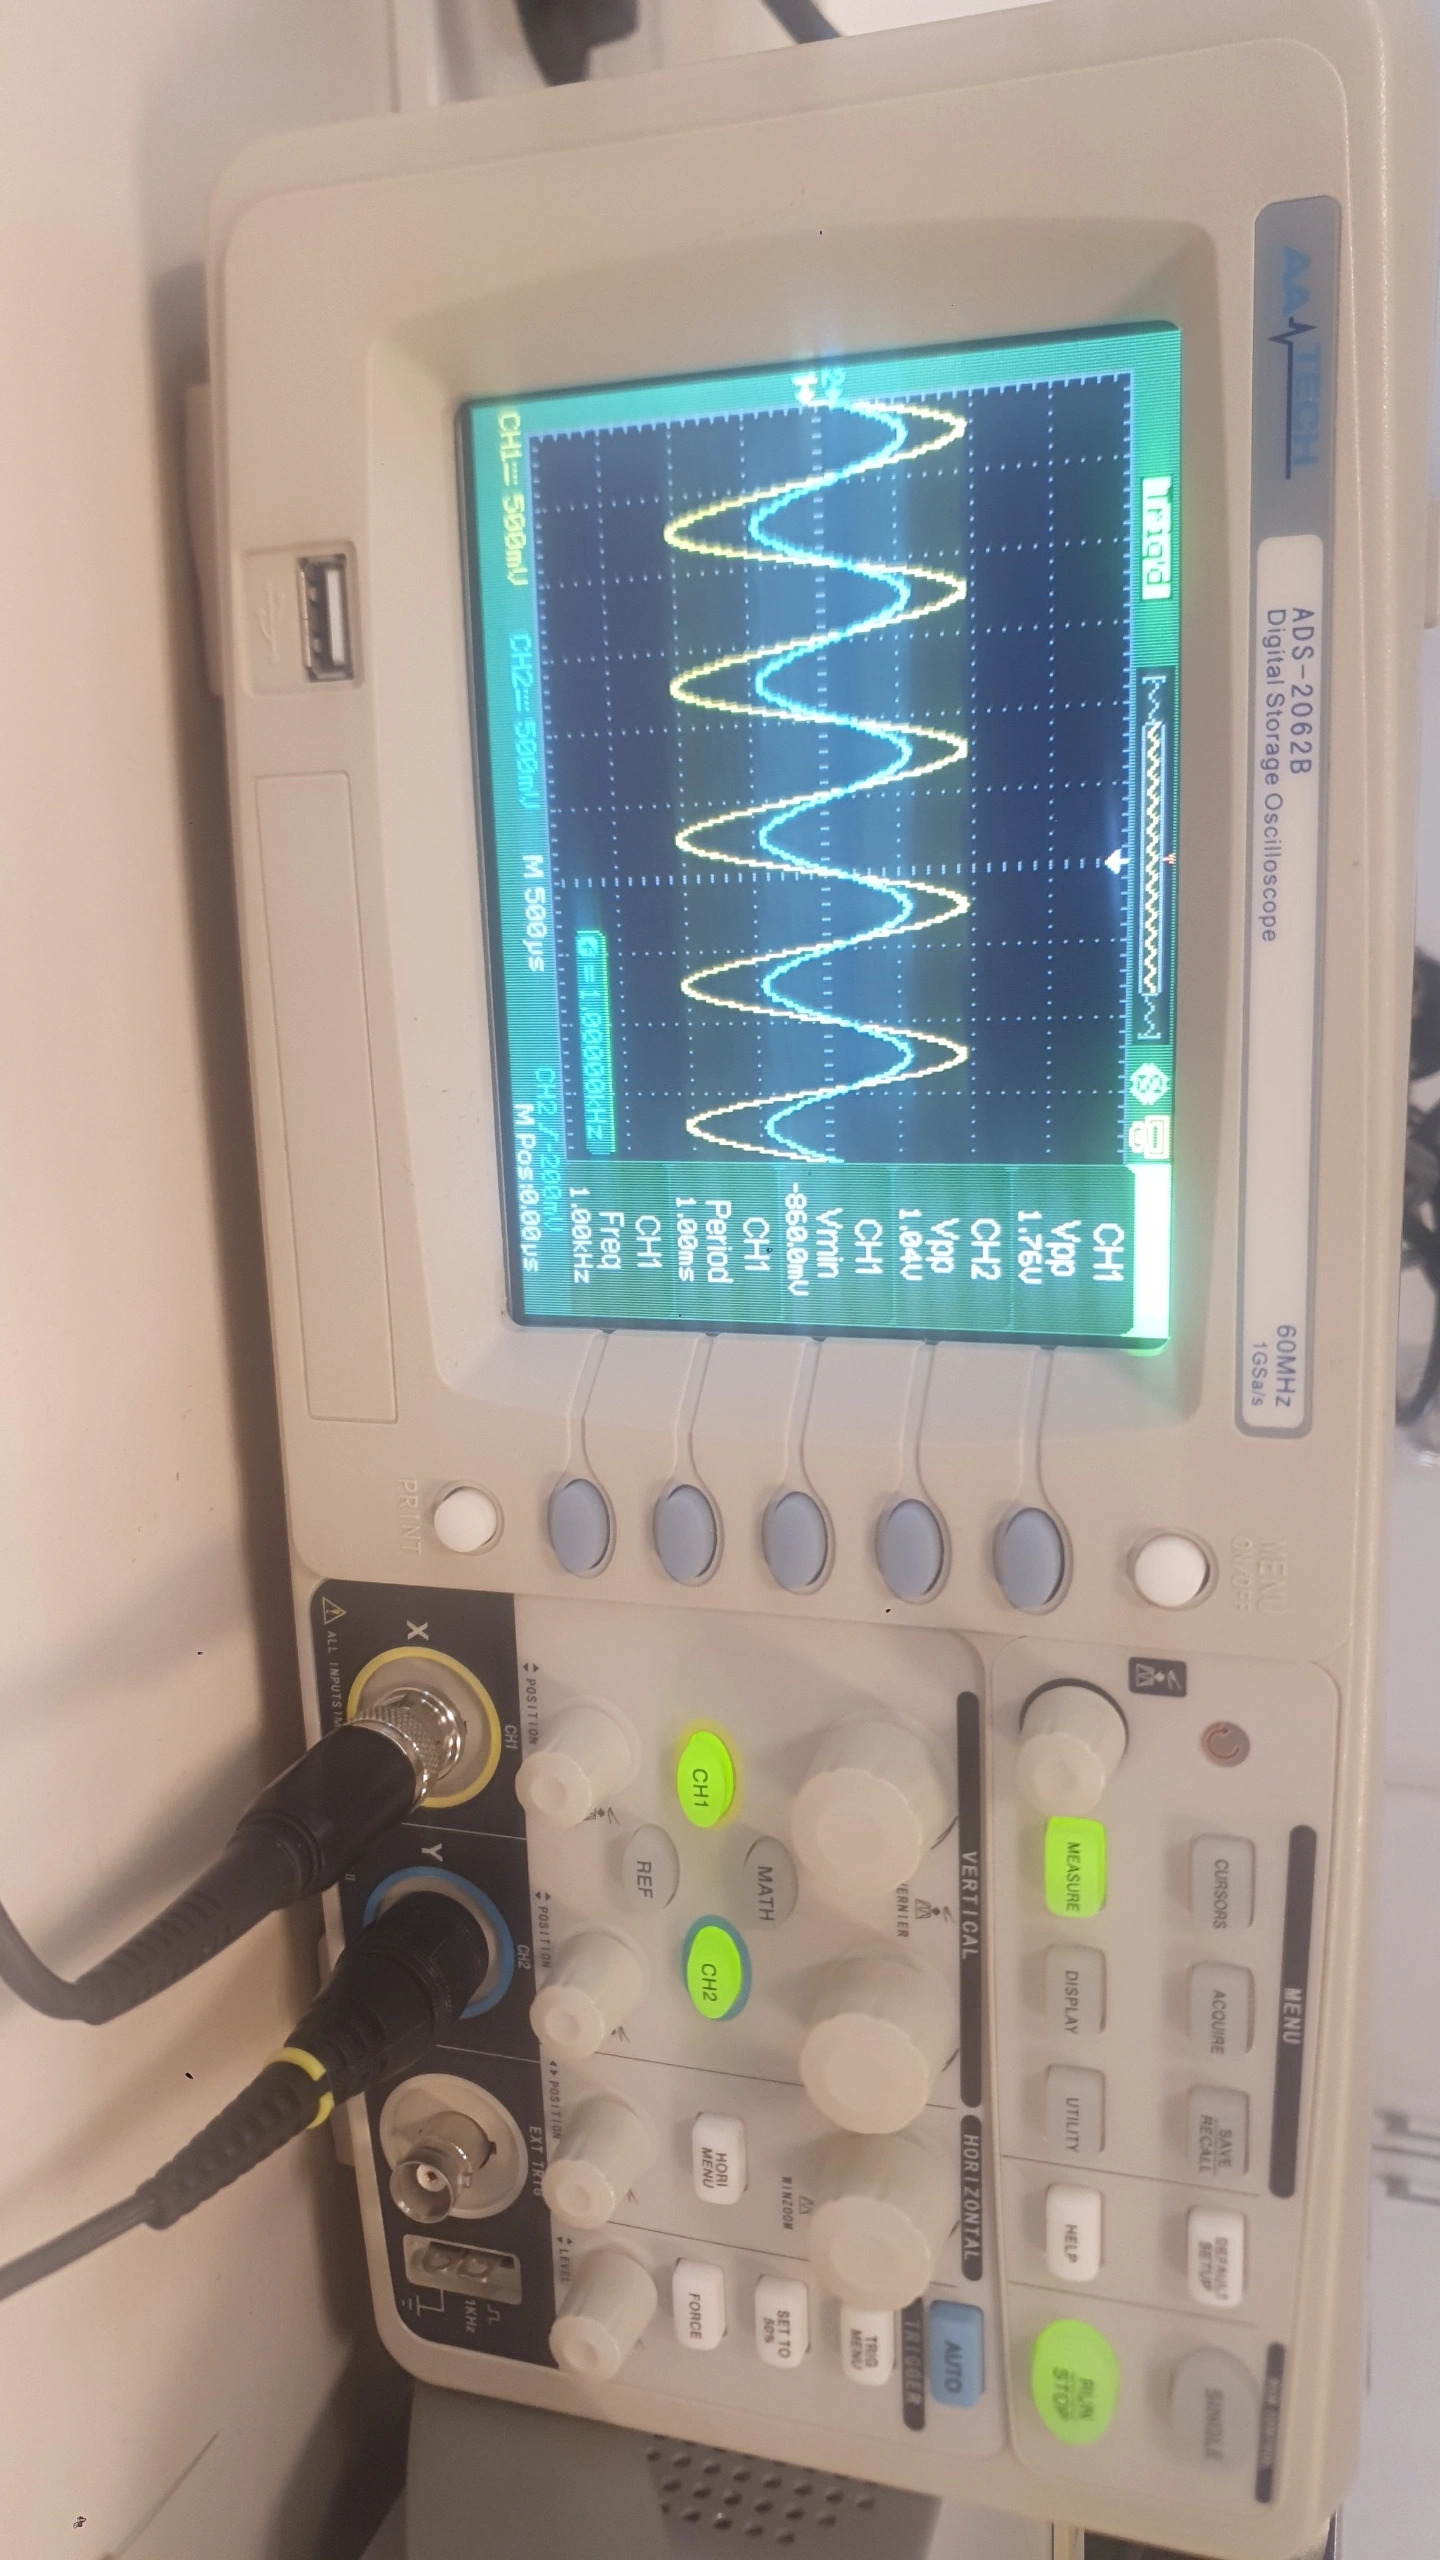
\includegraphics[scale=0.15,angle=90]{images/Lab1_figure1}
      \caption{$V_{AC}$ Yellow Wave Channel - $V_{BC}$ Blue Wave Channel}
      \label{fig:waveform}
  \end{figure}
  \end{itemize}
  
\end{enumerate}


\newpage
\paragraph{\textbf{1.2.2.2 Task 2.2}}  
Using the same experimental setup and replacing the necessary $ 1\text{k} \Omega $ resistors with $ 22\text{k} \Omega $ and $ 33\text{k} \Omega $ resistors, the second circuit should be constructed accordingly.  

Following the same measurement steps outlined in \textbf{Task 2.1}, the observed waveform is presented in the figure below:  

\begin{figure}[h]
  \centering
  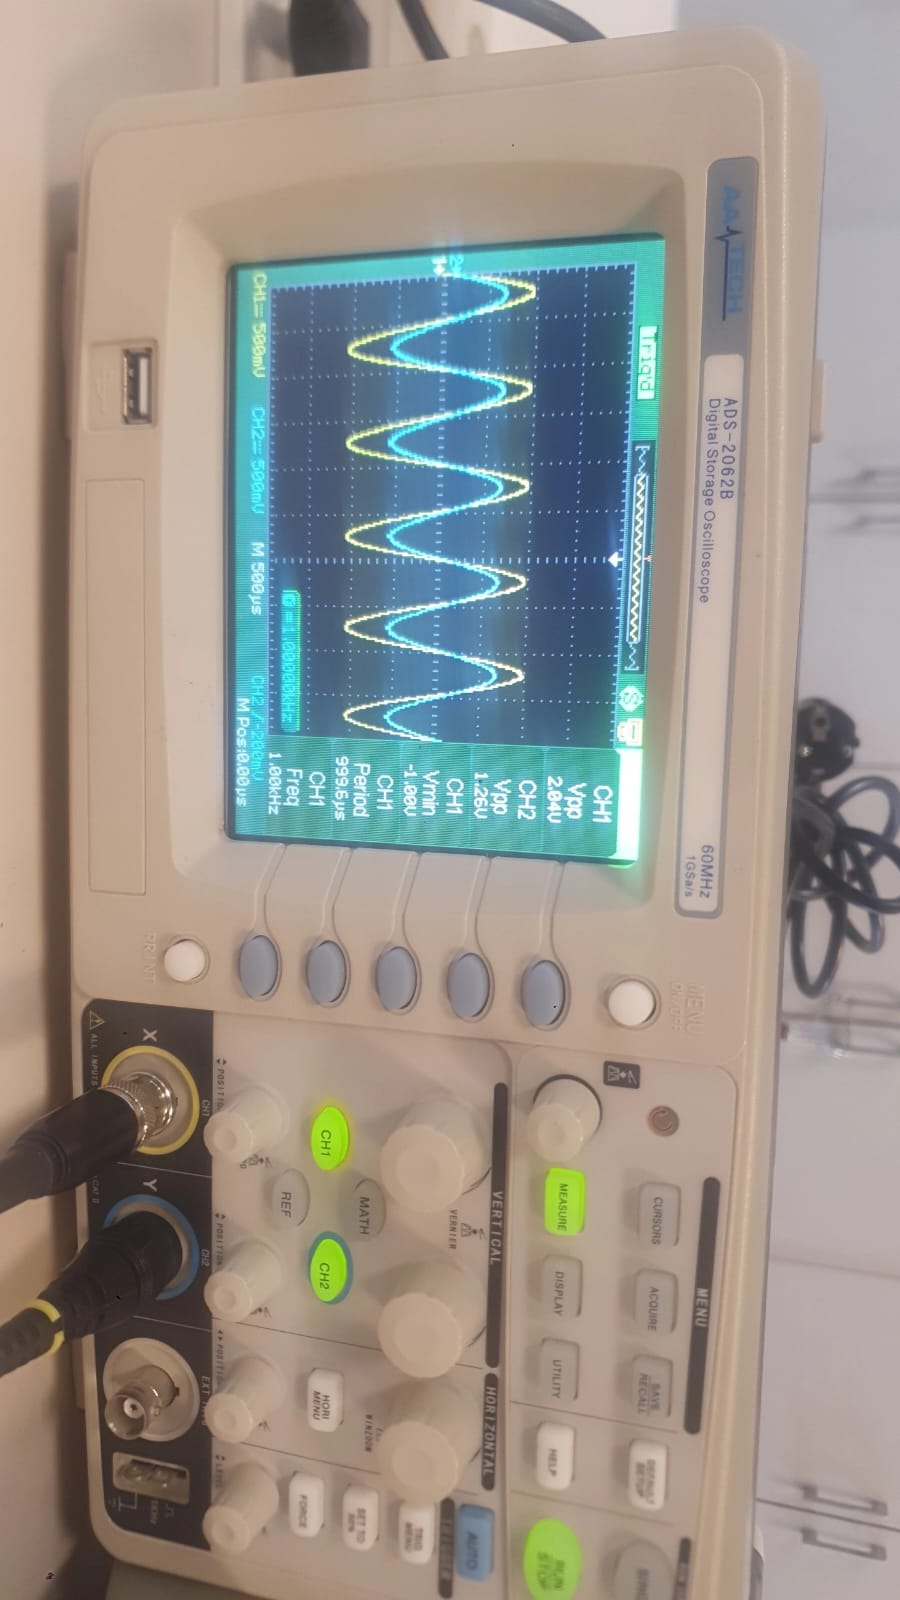
\includegraphics[scale=0.25, angle=90]{images/Lab1_figure2}
  \caption{$V_{AC}$ Yellow Wave Channel - $V_{BC}$ Blue Wave Channel}
  \label{fig:waveform}
\end{figure}



\section{Conclusion}
  


  In Task 1, as seen in Tables 2 and 3, the measured voltage and current values are closely aligned with the theoretical calculations, confirming the accuracy of Kirchhoff’s Current Law (KCL) and Kirchhoff’s Voltage Law (KVL) in circuit analysis. Minor discrepancies between the calculated and measured values may be attributed to component tolerances, contact resistance, or measurement limitations of the multimeter. Overall, the results validate the expected electrical behavior of the circuit.


  In Task 2, the sinusoidal waveforms and voltage levels were analyzed under different resistor configurations. The measured voltage values closely aligned with theoretical expectations, demonstrating the validity of the voltage divider principle. However, minor discrepancies were observed, which can be attributed to factors such as oscilloscope calibration drift, external noise, resistor tolerances, or improper contact on the breadboard.

\end{document}
